%!TEX root = start.TEX
\section{Propuesta o tema central de la tesis}
\frame{
\begin{block}
{\Large{Datos para el entrenamiento}}
\end{block}
%\vskip 0.5cm
	\begin{itemize}
	\item<1-> Señales de Tránsito de Alemania
	\begin{figure}[H]
				
				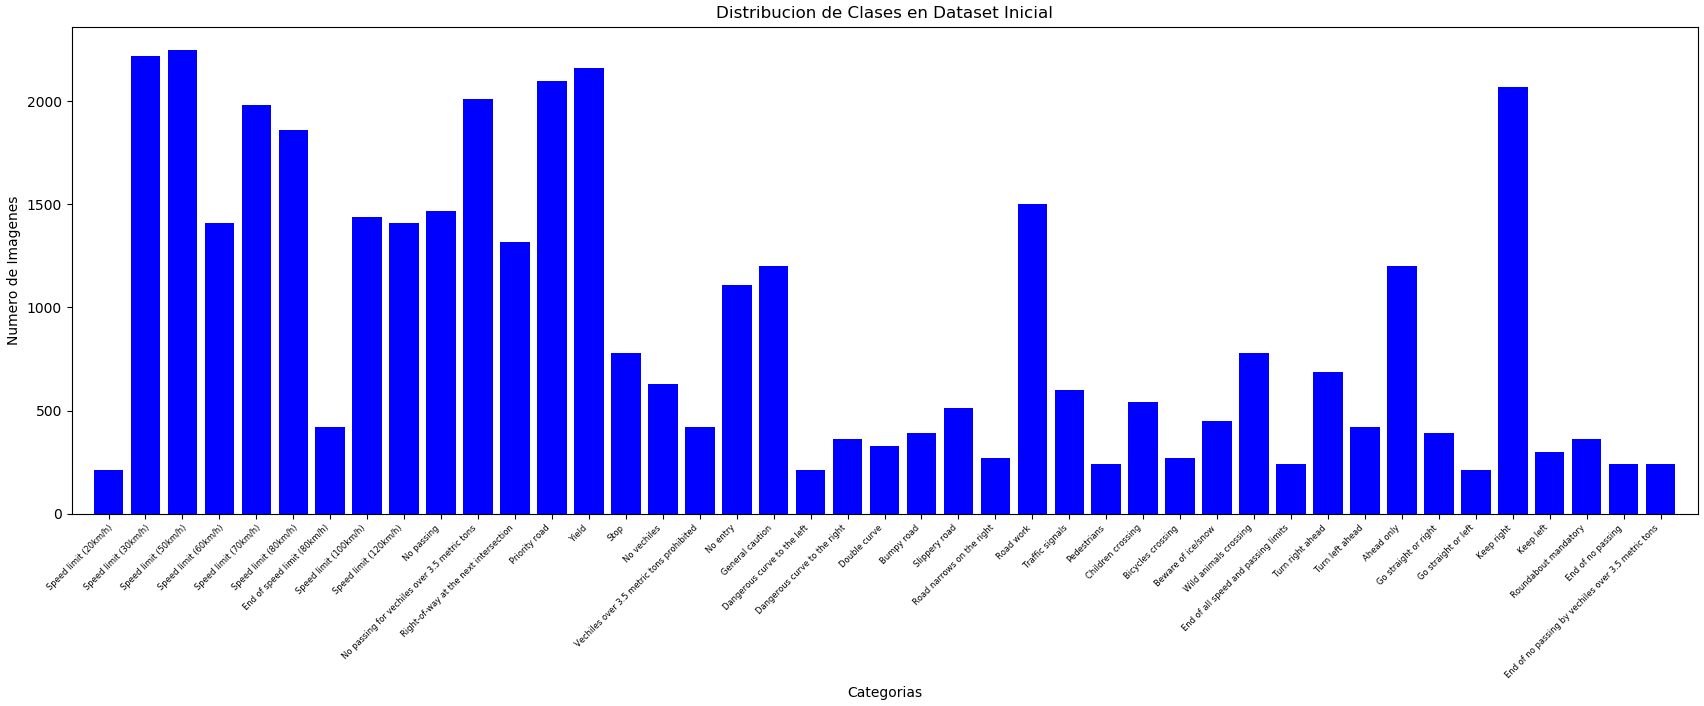
\includegraphics[width=0.9\textwidth,height=0.9\textheight,keepaspectratio]{images/desarrollo/histograms/initial39209}
				
				\begin{center}
				{\tiny{Distribución de ejemplos por señal para el entrenamiento(Total 39209)}}
				
			{\tiny {Fuente propia}}
				\end{center}
			\end{figure}
		
	\end{itemize}
}



\frame{
\begin{block}
{\Large{Datos para el entrenamiento}}
\end{block}
%\vskip 0.5cm
	\begin{itemize}

	\item<1->Señales de Tránsito de Perú
		\begin{figure}[H]
				\begin{center}
				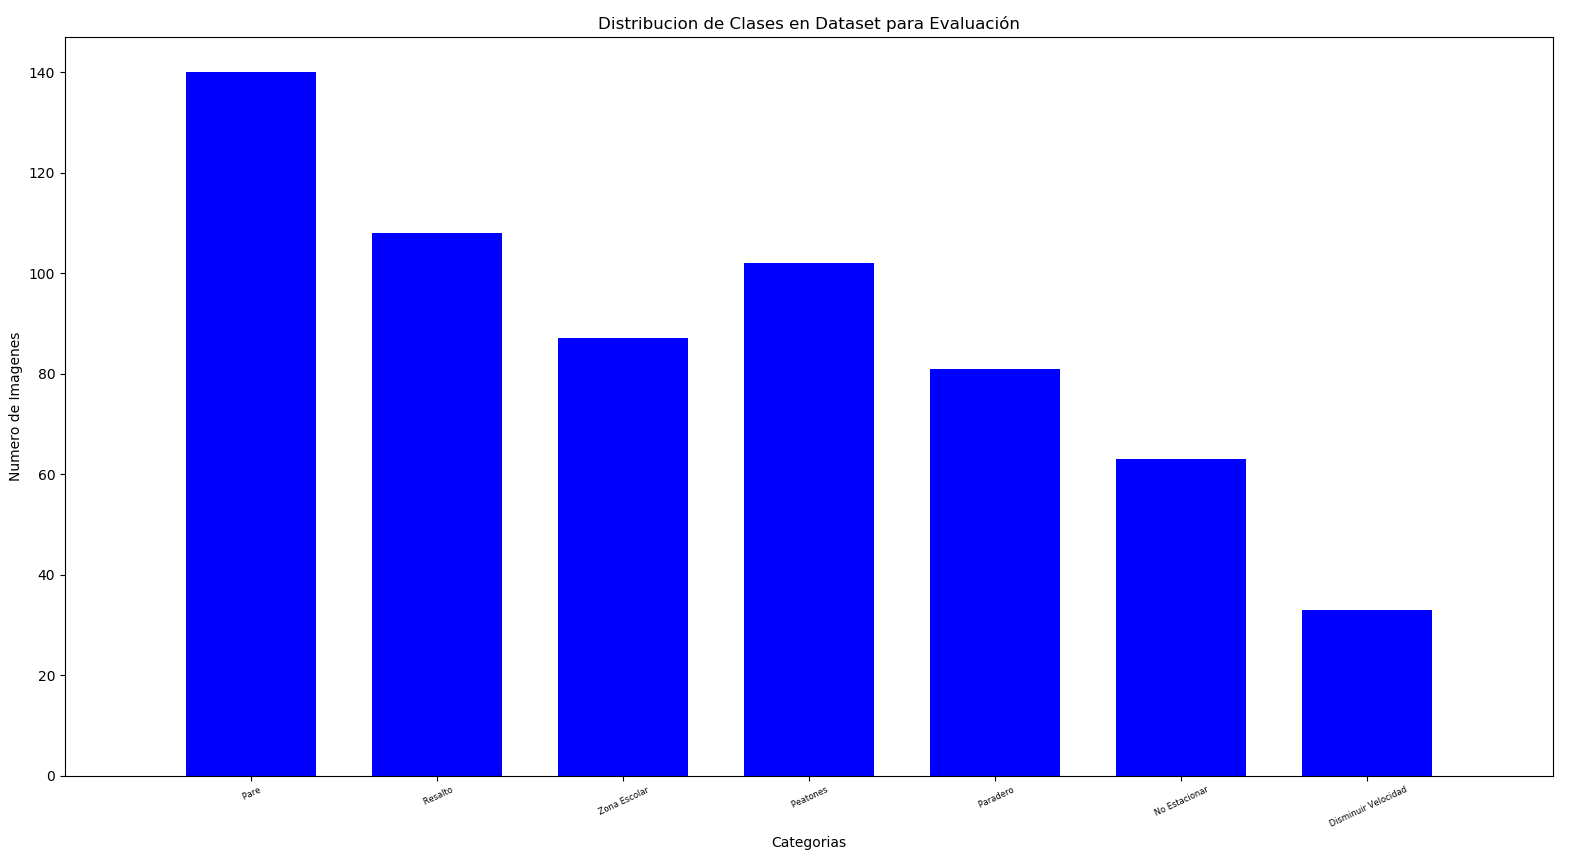
\includegraphics[width=0.9\textwidth,height=0.9\textheight,keepaspectratio]{images/desarrollo/histograms/inicioTrain614}
				\end{center}
				\begin{center}
				{\tiny{Distribución de ejemplos por señal para el entrenamiento(Total 614)}}
				
			{\tiny{Fuente propia}}
				\end{center}
			\end{figure}
	\end{itemize}
}




\frame{
\begin{block}
{\Large{Datos para la Evaluación}}
\end{block}
%\vskip 0.5cm
	\begin{itemize}
	\item<1-> Señales de Tránsito de Alemania (12630 imágenes)
	\begin{figure}[H]
				
				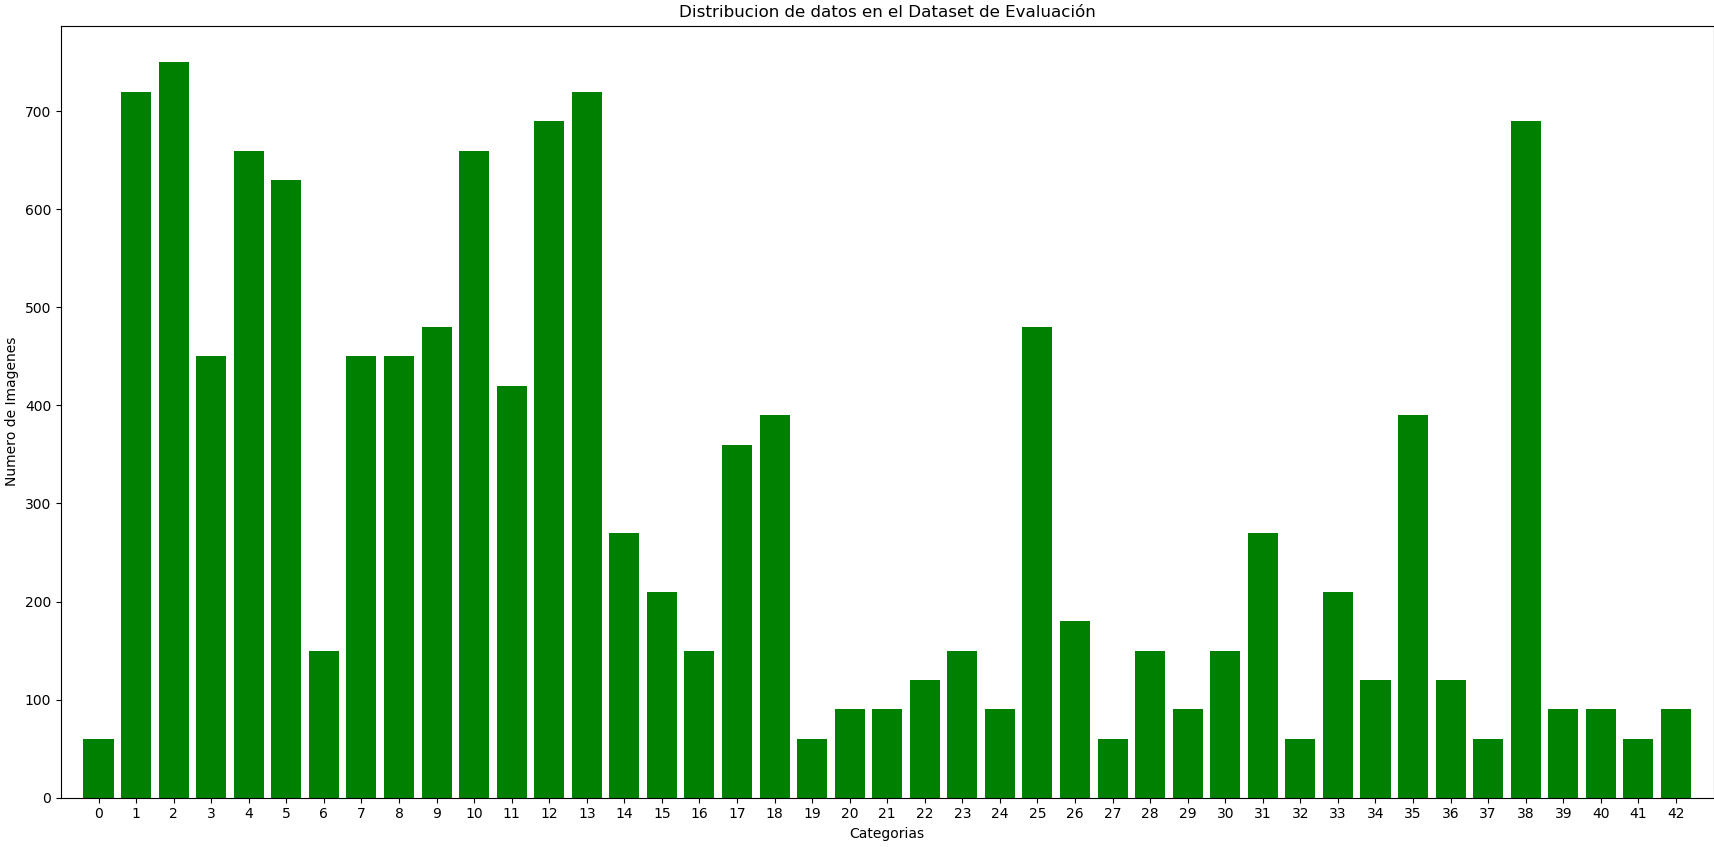
\includegraphics[width=0.9\textwidth,height=0.9\textheight,keepaspectratio]{images/desarrollo/histograms/initialTest12630}
				
				\begin{center}
				{\tiny{Distribución de ejemplos por señal para la evaluación - Alemania}}
				
			{\tiny {Fuente propia}}
				\end{center}
			\end{figure}
		
	\end{itemize}
}



\frame{
\begin{block}
{\Large{Datos para la Evaluación}}
\end{block}
%\vskip 0.5cm
	\begin{itemize}

	\item<1->Señales de Tránsito de Perú (4698 imágenes)
		\begin{figure}[H]
				\begin{center}
				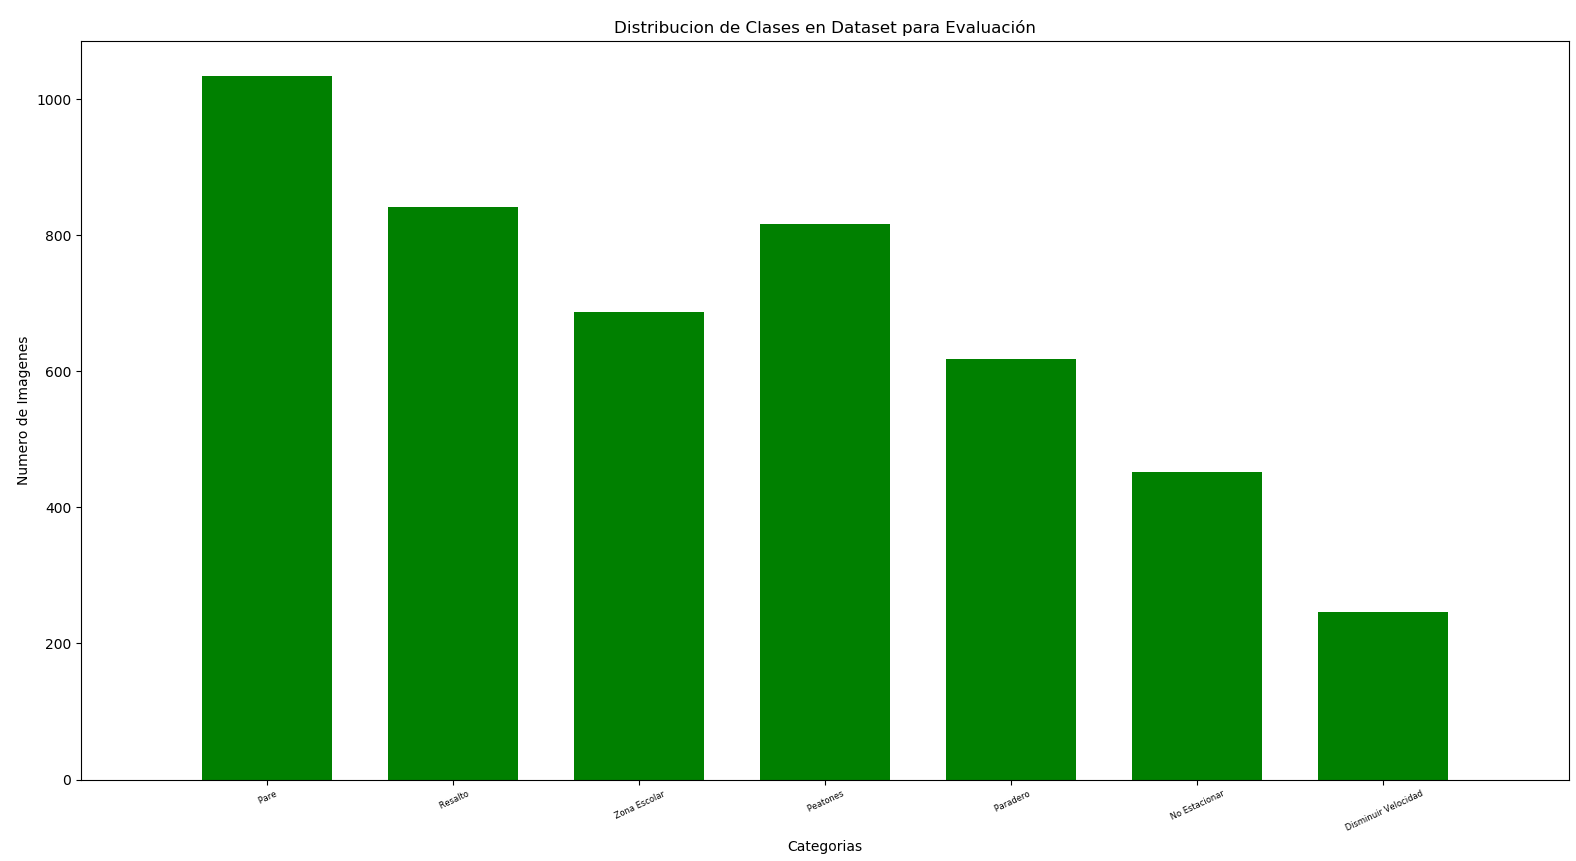
\includegraphics[width=0.9\textwidth,height=0.9\textheight,keepaspectratio]{images/desarrollo/histograms/PeruinitialTest4698}
				\end{center}
				\begin{center}
				{\tiny{Distribución de ejemplos por señal para la evaluación - Perú}}
				
			{\tiny{Fuente propia}}
				\end{center}
			\end{figure}
	\end{itemize}
}


%--------------------------------------Data Augmentation----------

\frame{
\begin{block}
{\Large{Proceso de Aumento de Datos(Data Augmentation)}}
\end{block}
	

	 \begin{enumerate}%\addtocounter{enumi}{2}
	\item Flipping
	\begin{multicols}{2}
				
				\underline{Flipping horizontal:}
				\begin{figure}[H]
					\begin{center}
					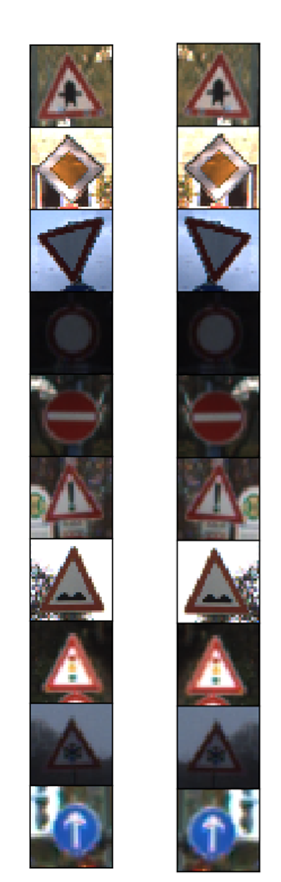
\includegraphics[width=0.7\textwidth,height=0.65\textheight,keepaspectratio]{images/desarrollo/Augment/flippedHorizontally}
					\end{center}
					%\begin{center}\tiny{Imágenes volteadas horizontalmente}\end{center}
					
				\end{figure}

			%second column
			
				\underline{Flipping Vertical:}
				\begin{figure}[H]
					\begin{center}
					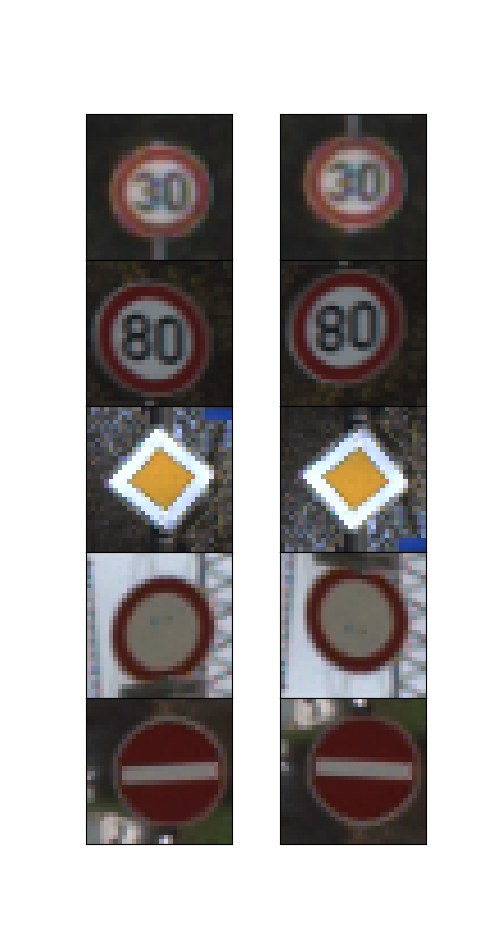
\includegraphics[width=0.7\textwidth,height=0.65\textheight,keepaspectratio]{images/desarrollo/Augment/flippableVertically}
					\end{center}
					%\begin{center}\tiny{Imágenes volteadas verticalmente}\end{center}

				\end{figure}

			\end{multicols}
	\end{enumerate}
}

\frame{
\begin{block}
{\Large{Proceso de Aumento de Datos(Data Augmentation)}}
\end{block}


	\underline{Flipping Horizontal y Vertical:}
			\begin{figure}[H]
				\begin{center}
				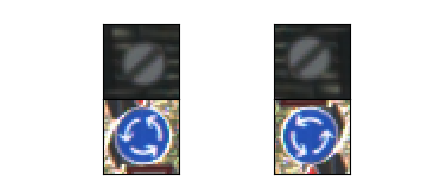
\includegraphics[width=0.7\textwidth,height=0.65\textheight,keepaspectratio ]{images/desarrollo/Augment/flippable_both}
				\end{center}
				
				%\tiny{Imágenes que volteadas horizontal o verticalmente, cambian su categoría}
				
			
			\end{figure}

}

\frame{
\begin{block}
{\Large{Proceso de Aumento de Datos(Data Augmentation)}}
\end{block}
	

	Incluso, hay signos que luego de voltearse, deben clasificarse como un signo de alguna otra clase. Esto sigue siendo útil, ya que podemos utilizar los datos de estas clases para ampliar sus contrapartes.
			\begin{figure}[H]
				\begin{center}
				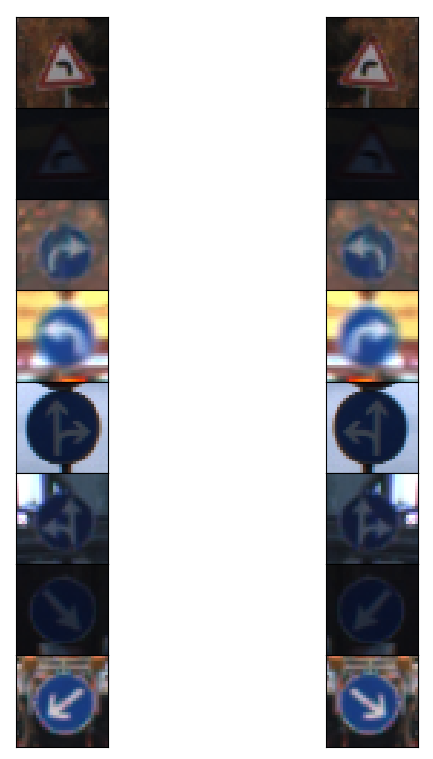
\includegraphics[width=0.7\textwidth,height=0.65\textheight,keepaspectratio ]{images/desarrollo/Augment/cross_flippable}
				\end{center}
				
				%\tiny{Imágenes que volteadas horizontal o verticalmente, cambian su categoría}
				
			
			\end{figure}

}



\frame{
\begin{block}
{\Large{Proceso de Aumento de Datos(Data Augmentation)}}
\end{block}
	

	Finalmente obtenemos una nueva distribución de datos luego de haber aplicado flipping a ciertas imagenes. Esta distribución consta de 63538 imágenes.
			\begin{figure}[H]
				\begin{center}
				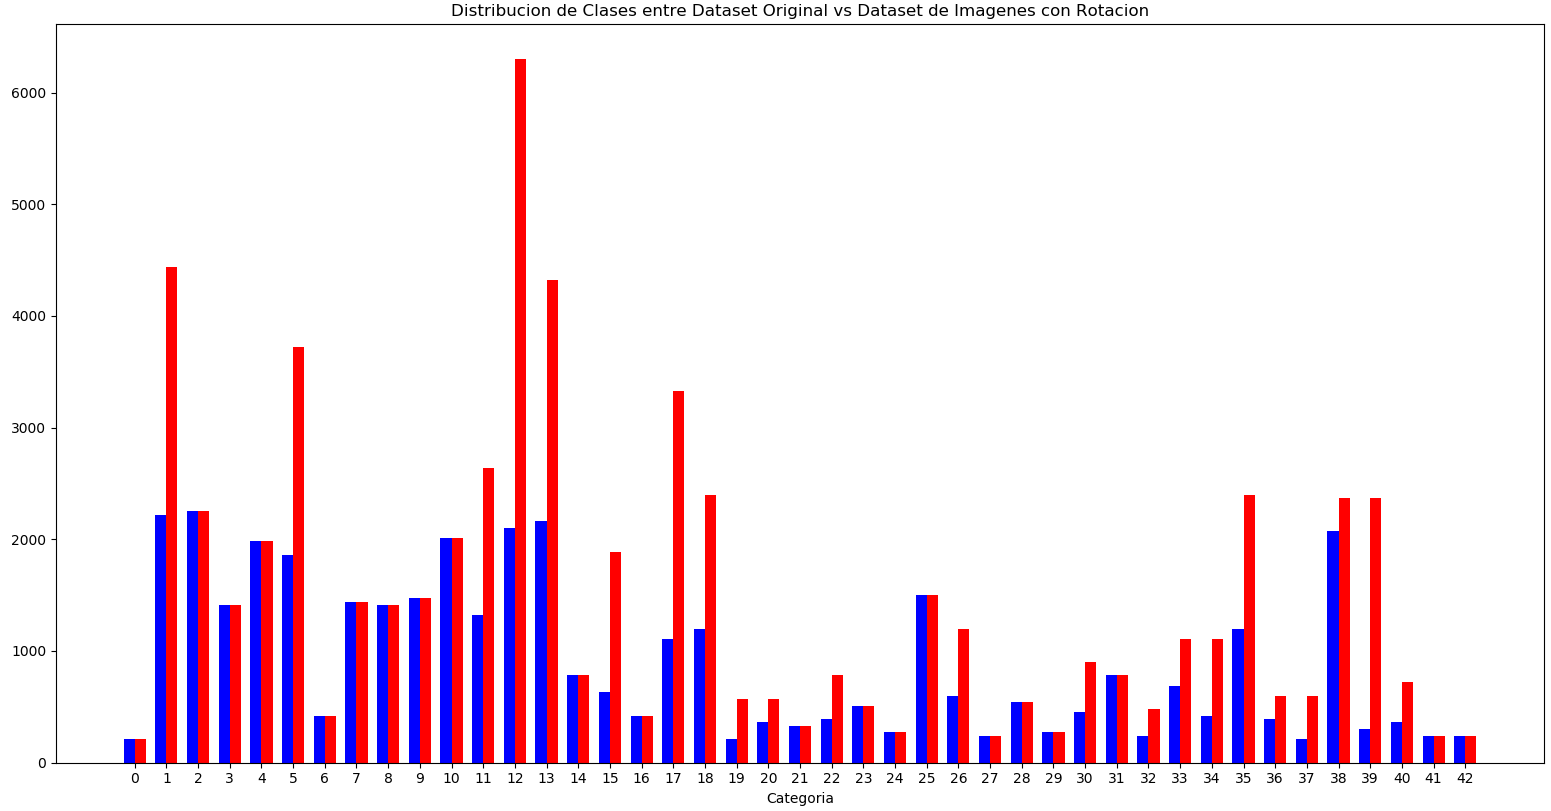
\includegraphics[width=0.8\textwidth,height=0.8\textheight,keepaspectratio]{images/desarrollo/histograms/train_flipped63538}
				\end{center}
				
				\vspace{-0.5em}
				{\tiny{Distribución de categoría, luego de aplicar el Flip(en sus distintos tipos)- Señales de Alemania}}

			\end{figure}
}


\frame{
\begin{block}
{\Large{Proceso de Aumento de Datos(Data Augmentation)}}
\end{block}
	


	 \begin{enumerate}\addtocounter{enumi}{1}
	 	\item Projection(Proyección)
			\begin{figure}[H]
				\begin{center}
				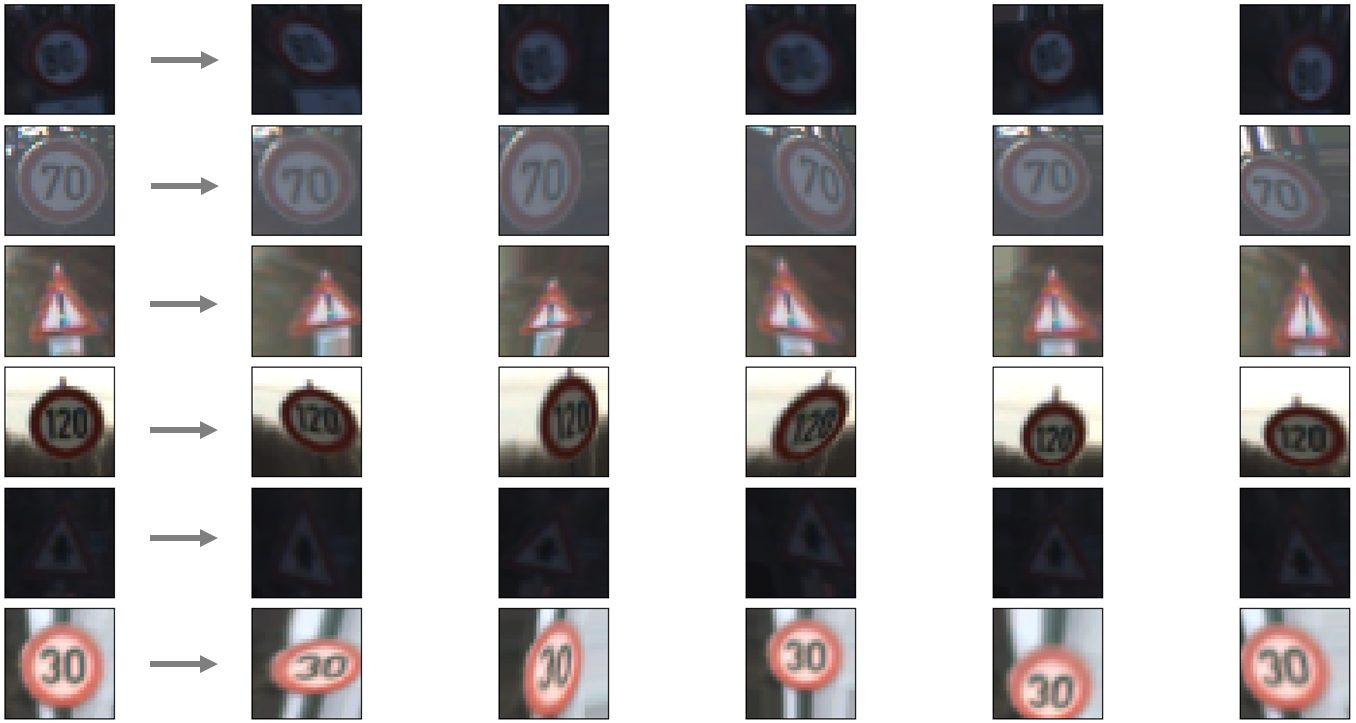
\includegraphics[width=0.8\textwidth,height=0.8\textheight,keepaspectratio]{images/desarrollo/Augment/projection_transform}
				\end{center}
				
				
				{\tiny{Ejemplo de cinco proyecciones por cada imagen - Dataset Alemania}}

			\end{figure}
		\end{enumerate}
}






\frame{
\begin{block}
{\Large{Proceso de Aumento de Datos(Data Augmentation)}}
\end{block}
	


	 \begin{enumerate}\addtocounter{enumi}{2}
	 	\item Rotation(Rotación)
			\begin{figure}[H]
				\begin{center}
				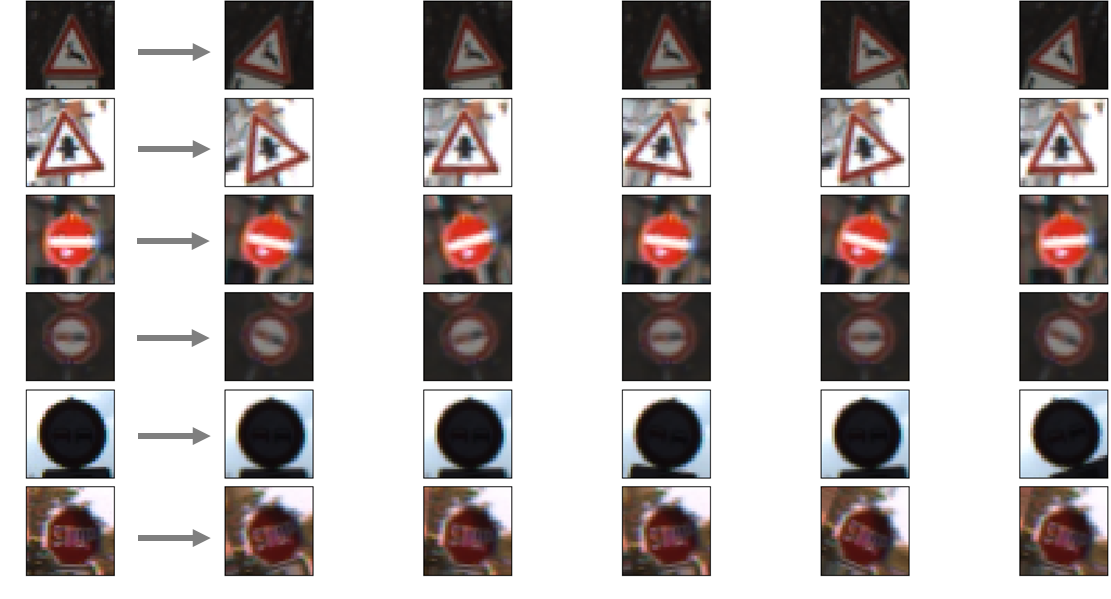
\includegraphics[width=0.8\textwidth,height=0.8\textheight,keepaspectratio]{images/desarrollo/Augment/fixedrotation}
				\end{center}
				
				
				{\tiny{Ejemplo de cinco rotaciones por cada imagen - Dataset Alemania}}

			\end{figure}
		\end{enumerate}
}



\frame{
\begin{block}
{\Large{Proceso de Aumento de Datos(Data Augmentation)}}
\end{block}
	


	 \begin{enumerate}\addtocounter{enumi}{3}
	 	\item Zoom
			\begin{figure}[H]
				\begin{center}
				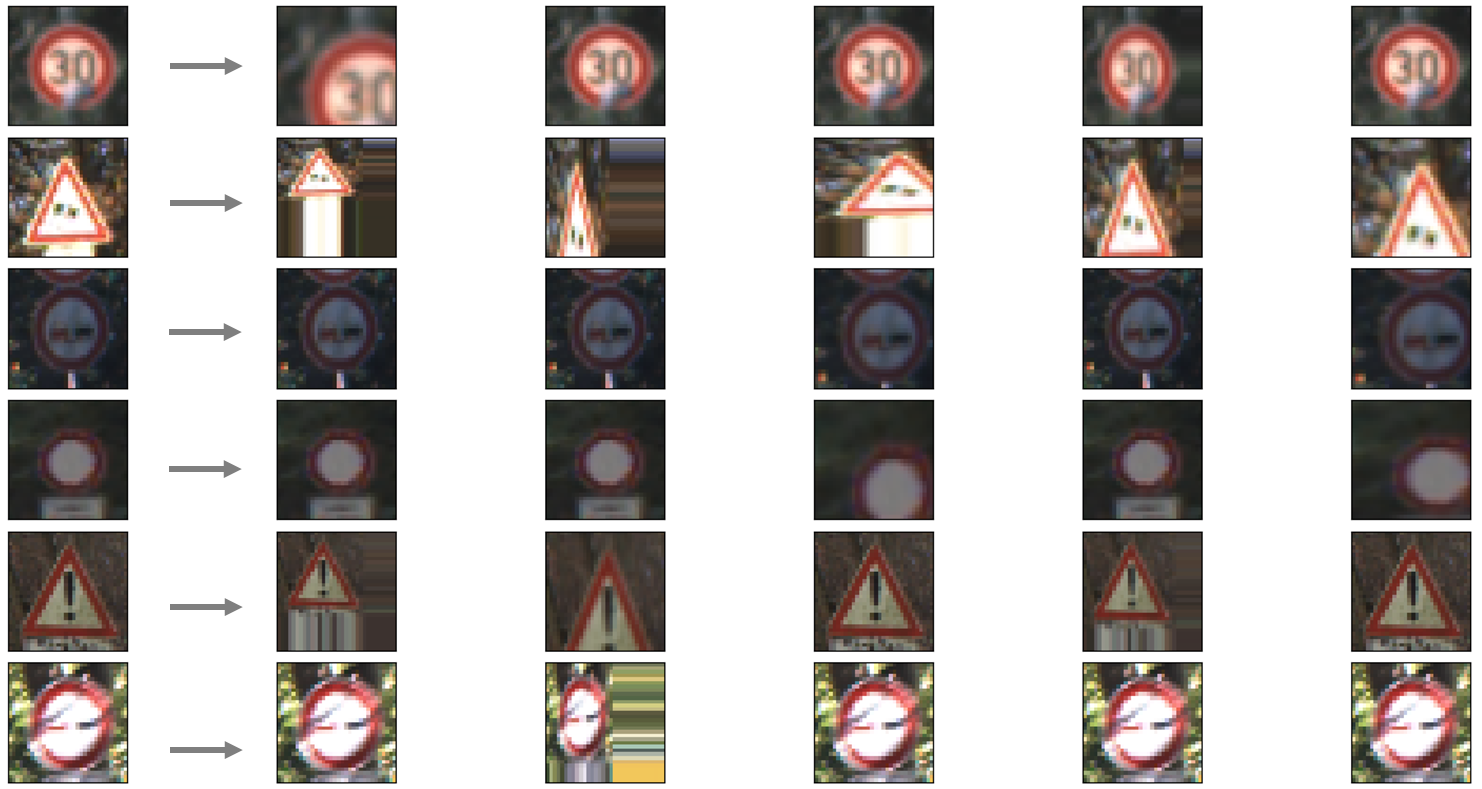
\includegraphics[width=0.8\textwidth,height=0.8\textheight,keepaspectratio]{images/desarrollo/Augment/zoom_inv}
				\end{center}
				
				
				{\tiny{Ejemplo de cinco aplicaciones de zoom(in/out) por cada imagen - Dataset Alemania}}

			\end{figure}
		\end{enumerate}
}

\frame{
\begin{block}
{\Large{Proceso de Aumento de Datos(Data Augmentation)}}
\end{block}
	


	 \begin{enumerate}\addtocounter{enumi}{4}
	 	\item Equalizacion del histograma
			\begin{figure}[H]
				\begin{center}
				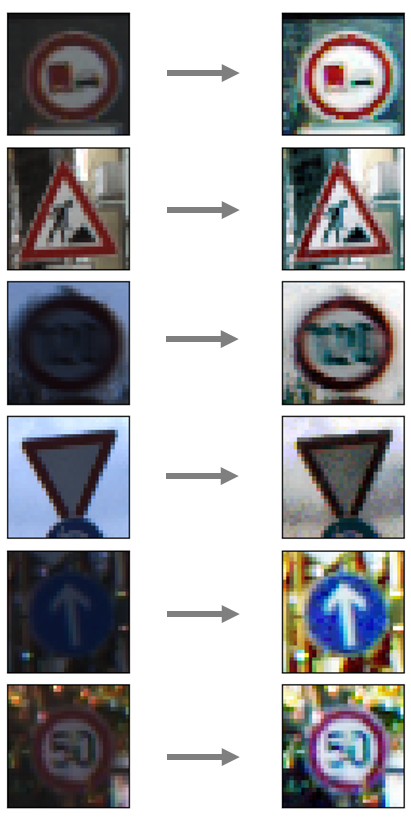
\includegraphics[width=0.8\textwidth,height=0.8\textheight,keepaspectratio]{images/desarrollo/Augment/equalize_hist2_wo_Norm_woRepetition}
				\end{center}
				{\tiny{Distribución eficaz de los valores de intensidad más frecuentes}}
			\end{figure}
		\end{enumerate}
}

%------------------------------------------------------------------



\frame{
\begin{block}
{\Large{Dataset final }}
\end{block}
%\vskip 0.5cm
	\begin{itemize}
	\item<1-> Señales de Tránsito de Alemania (270900 imágenes)
	\begin{figure}[H]
				
				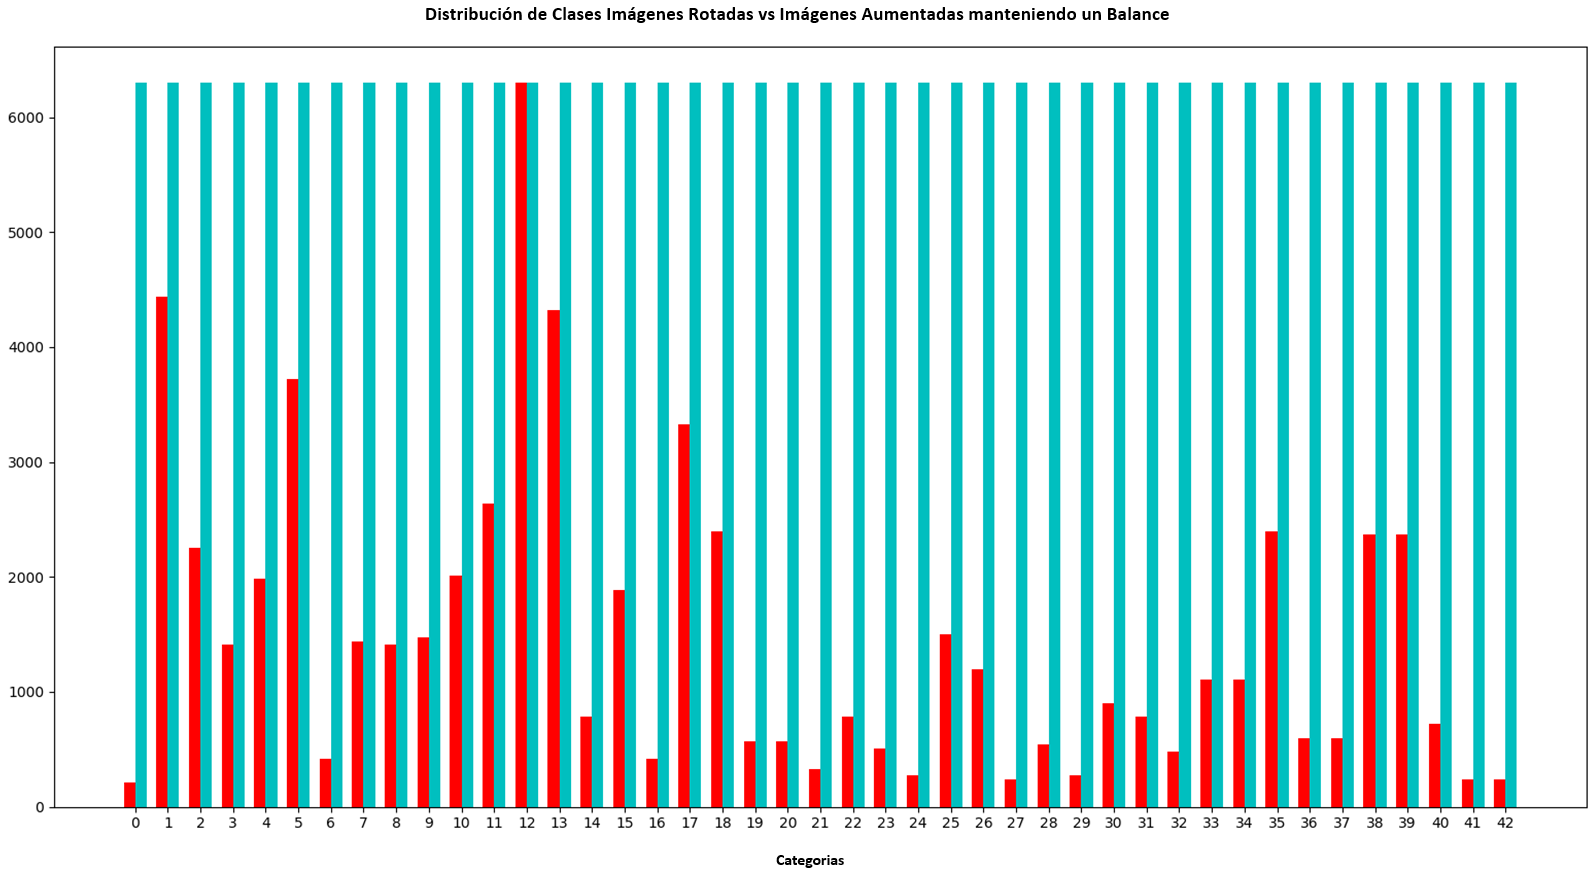
\includegraphics[width=0.9\textwidth,height=0.9\textheight,keepaspectratio]{images/desarrollo/histograms/train_extended_balanced270900}

			\end{figure}
		
	\end{itemize}
}

\frame{
\begin{block}
{\Large{Dataset final }}
\end{block}
%\vskip 0.5cm
	\begin{itemize}

	\item<1->Señales de Tránsito de Perú (31314 imágenes)
		\begin{figure}[H]
				\begin{center}
				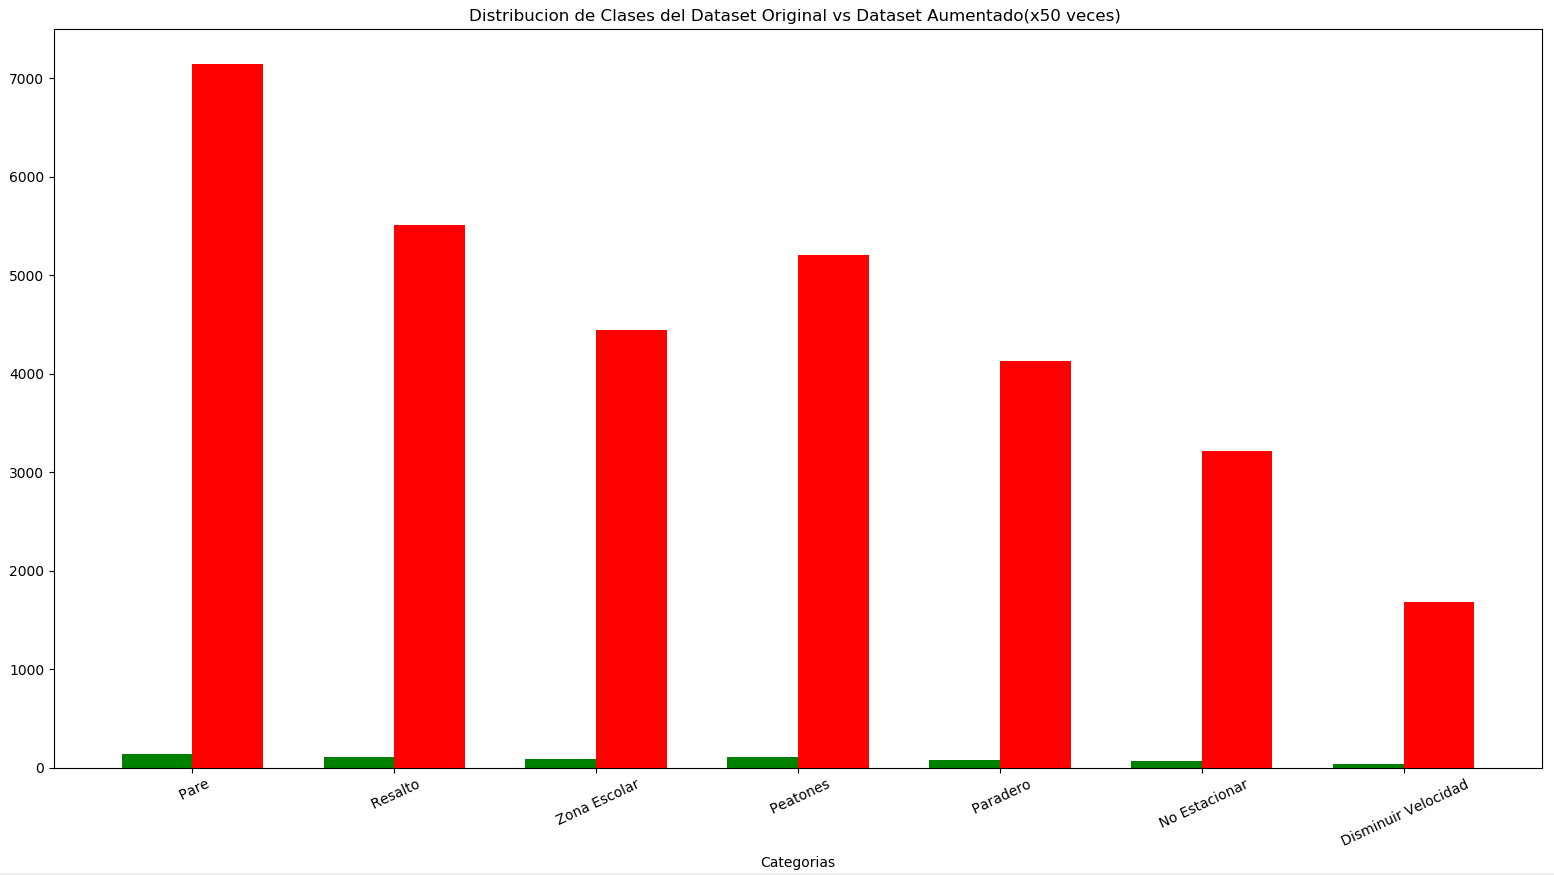
\includegraphics[width=0.9\textwidth,height=0.9\textheight,keepaspectratio]{images/desarrollo/histograms/train_extended_per_51_31314}
				\end{center}
			\end{figure}
	\end{itemize}
}



\frame{
\begin{block}
{\Large{Pre-procesamiento de Imágenes(Normalization) }}
\end{block}
%\vskip 0.5cm
	\begin{itemize}

	\item<1->La técnica utilizada CLAHE es un algoritmo para la mejora del contraste local, que utiliza histogramas calculados sobre diferentes regiones en una imagen.
	\vskip 0.2cm
	\item<2->Difiere de la ecualización de histograma ordinaria en el sentido de que el método adaptativo computa varios histogramas, cada uno correspondiente a una sección distinta de la imagen, y los utiliza para redistribuir los valores de luminosidad de la imagen.
	\vskip 0.2cm
	\item<3->Mejora el nivel de visibilidad de una imagen o video con niebla ya que permite mejorar los detalles locales incluso en regiones que son más oscuras o más claras que la mayoría de regiones de la imagen. \citep{CLAHE}
		\begin{figure}[H]
				\begin{center}
				
\includegraphics[width=0.9\textwidth,height=0.9\textheight,keepaspectratio]{images/desarrollo/Normalization_Processing/norm_test2}
				\end{center}
			\end{figure}
	\end{itemize}
}


\frame{
\begin{block}
{\Large{Pre-procesamiento de Imágenes(Normalization) }}
\end{block}
%\vskip 0.5cm
	\begin{itemize}

	\item<1->Pierre Sermanet y Yann LeCun mencionaron en su artículo \citep{LeCun}, que el uso de canales de color no pareció mejorar mucho las cosas. Además, debido a diversas condiciones o problemas de iluminación, no es adecuado procesar directamente las imágenes que se capturan a través de la cámara o sensores de imágenes, es por ello que en esta investigación {\bf se usará un solo canal} en el modelo, es decir las imágenes estarán en escala de grises en lugar de tener 3 canales de colores.
	
		\begin{figure}[H]
				\begin{center}
				
\includegraphics[width=0.9\textwidth,height=0.9\textheight,keepaspectratio]{images/desarrollo/Normalization_Processing/proc_test2}
				\end{center}
			\end{figure}
	\end{itemize}
}
